%% infiPaper.tex
%% 2008/12/09
%% by Daniel Kirchner, Alex Lotz, Andreas Steck


\documentclass[11pt, journal]{IEEEtran}
%\documentclass[conference]{IEEEtran}
%
% If IEEEtran.cls has not been installed into the LaTeX system files,
% manually specify the path to it like:
% \documentclass[journal]{../sty/IEEEtran}


% Some very useful LaTeX packages include:
% (uncomment the ones you want to load)

%% this is to get centered captions (figure)
\makeatletter
\long\def\@makecaption#1#2{\ifx\@captype\@IEEEtablestring%
\footnotesize\begin{center}{\normalfont\footnotesize #1}\\
{\normalfont\footnotesize\scshape #2}\end{center}%
\@IEEEtablecaptionsepspace
\else
\@IEEEfigurecaptionsepspace
\setbox\@tempboxa\hbox{\normalfont\footnotesize {#1.}~~ #2}%
\ifdim \wd\@tempboxa >\hsize%
\setbox\@tempboxa\hbox{\normalfont\footnotesize {#1.}~~ }%
\parbox[t]{\hsize}{\normalfont\footnotesize \noindent\unhbox\@tempboxa#2}%
\else
\hbox to\hsize{\normalfont\footnotesize\hfil\box\@tempboxa\hfil}\fi\fi}
\makeatother


% *** MISC UTILITY PACKAGES ***
%
%\usepackage{ifpdf}
% Heiko Oberdiek's ifpdf.sty is very useful if you need conditional
% compilation based on whether the output is pdf or dvi.
% usage:
% \ifpdf
%   % pdf code
% \else
%   % dvi code
% \fi
% The latest version of ifpdf.sty can be obtained from:
% http://www.ctan.org/tex-archive/macros/latex/contrib/oberdiek/
% Also, note that IEEEtran.cls V1.7 and later provides a builtin
% \ifCLASSINFOpdf conditional that works the same way.
% When switching from latex to pdflatex and vice-versa, the compiler may
% have to be run twice to clear warning/error messages.


% *** CITATION PACKAGES ***
%
\usepackage{cite}
% cite.sty was written by Donald Arseneau
% V1.6 and later of IEEEtran pre-defines the format of the cite.sty package
% \cite{} output to follow that of IEEE. Loading the cite package will
% result in citation numbers being automatically sorted and properly
% "compressed/ranged". e.g., [1], [9], [2], [7], [5], [6] without using
% cite.sty will become [1], [2], [5]--[7], [9] using cite.sty. cite.sty's
% \cite will automatically add leading space, if needed. Use cite.sty's
% noadjust option (cite.sty V3.8 and later) if you want to turn this off.
% cite.sty is already installed on most LaTeX systems. Be sure and use
% version 4.0 (2003-05-27) and later if using hyperref.sty. cite.sty does
% not currently provide for hyperlinked citations.
% The latest version can be obtained at:
% http://www.ctan.org/tex-archive/macros/latex/contrib/cite/
% The documentation is contained in the cite.sty file itself.


% *** GRAPHICS RELATED PACKAGES ***
%
\ifCLASSINFOpdf
  \usepackage[pdftex]{graphicx}
  % declare the path(s) where your graphic files are
  % \graphicspath{{../pdf/}{../jpeg/}}
  % and their extensions so you won't have to specify these with
  % every instance of \includegraphics
  % \DeclareGraphicsExtensions{.pdf,.jpeg,.png}
\else
  % or other class option (dvipsone, dvipdf, if not using dvips). graphicx
  % will default to the driver specified in the system graphics.cfg if no
  % driver is specified.
  % \usepackage[dvips]{graphicx}
  % declare the path(s) where your graphic files are
  % \graphicspath{{../eps/}}
  % and their extensions so you won't have to specify these with
  % every instance of \includegraphics
  % \DeclareGraphicsExtensions{.eps}
\fi
% graphicx was written by David Carlisle and Sebastian Rahtz. It is
% required if you want graphics, photos, etc. graphicx.sty is already
% installed on most LaTeX systems. The latest version and documentation can
% be obtained at: 
% http://www.ctan.org/tex-archive/macros/latex/required/graphics/
% Another good source of documentation is "Using Imported Graphics in
% LaTeX2e" by Keith Reckdahl which can be found as epslatex.ps or
% epslatex.pdf at: http://www.ctan.org/tex-archive/info/
%
% latex, and pdflatex in dvi mode, support graphics in encapsulated
% postscript (.eps) format. pdflatex in pdf mode supports graphics
% in .pdf, .jpeg, .png and .mps (metapost) formats. Users should ensure
% that all non-photo figures use a vector format (.eps, .pdf, .mps) and
% not a bitmapped formats (.jpeg, .png). IEEE frowns on bitmapped formats
% which can result in "jaggedy"/blurry rendering of lines and letters as
% well as large increases in file sizes.
%
% You can find documentation about the pdfTeX application at:
% http://www.tug.org/applications/pdftex


% *** MATH PACKAGES ***
%
%\usepackage[cmex10]{amsmath}
% A popular package from the American Mathematical Society that provides
% many useful and powerful commands for dealing with mathematics. If using
% it, be sure to load this package with the cmex10 option to ensure that
% only type 1 fonts will utilized at all point sizes. Without this option,
% it is possible that some math symbols, particularly those within
% footnotes, will be rendered in bitmap form which will result in a
% document that can not be IEEE Xplore compliant!
%
% Also, note that the amsmath package sets \interdisplaylinepenalty to 10000
% thus preventing page breaks from occurring within multiline equations. Use:
%\interdisplaylinepenalty=2500
% after loading amsmath to restore such page breaks as IEEEtran.cls normally
% does. amsmath.sty is already installed on most LaTeX systems. The latest
% version and documentation can be obtained at:
% http://www.ctan.org/tex-archive/macros/latex/required/amslatex/math/


% *** SPECIALIZED LIST PACKAGES ***
%
%\usepackage{algorithmic}
% algorithmic.sty was written by Peter Williams and Rogerio Brito.
% This package provides an algorithmic environment fo describing algorithms.
% You can use the algorithmic environment in-text or within a figure
% environment to provide for a floating algorithm. Do NOT use the algorithm
% floating environment provided by algorithm.sty (by the same authors) or
% algorithm2e.sty (by Christophe Fiorio) as IEEE does not use dedicated
% algorithm float types and packages that provide these will not provide
% correct IEEE style captions. The latest version and documentation of
% algorithmic.sty can be obtained at:
% http://www.ctan.org/tex-archive/macros/latex/contrib/algorithms/
% There is also a support site at:
% http://algorithms.berlios.de/index.html
% Also of interest may be the (relatively newer and more customizable)
% algorithmicx.sty package by Szasz Janos:
% http://www.ctan.org/tex-archive/macros/latex/contrib/algorithmicx/


% *** ALIGNMENT PACKAGES ***
%
%\usepackage{array}
% Frank Mittelbach's and David Carlisle's array.sty patches and improves
% the standard LaTeX2e array and tabular environments to provide better
% appearance and additional user controls. As the default LaTeX2e table
% generation code is lacking to the point of almost being broken with
% respect to the quality of the end results, all users are strongly
% advised to use an enhanced (at the very least that provided by array.sty)
% set of table tools. array.sty is already installed on most systems. The
% latest version and documentation can be obtained at:
% http://www.ctan.org/tex-archive/macros/latex/required/tools/


%\usepackage{mdwmath}
%\usepackage{mdwtab}
% Also highly recommended is Mark Wooding's extremely powerful MDW tools,
% especially mdwmath.sty and mdwtab.sty which are used to format equations
% and tables, respectively. The MDWtools set is already installed on most
% LaTeX systems. The lastest version and documentation is available at:
% http://www.ctan.org/tex-archive/macros/latex/contrib/mdwtools/


% IEEEtran contains the IEEEeqnarray family of commands that can be used to
% generate multiline equations as well as matrices, tables, etc., of high
% quality.


%\usepackage{eqparbox}
% Also of notable interest is Scott Pakin's eqparbox package for creating
% (automatically sized) equal width boxes - aka "natural width parboxes".
% Available at:
% http://www.ctan.org/tex-archive/macros/latex/contrib/eqparbox/


% *** SUBFIGURE PACKAGES ***
\usepackage[tight,footnotesize]{subfigure}
% subfigure.sty was written by Steven Douglas Cochran. This package makes it
% easy to put subfigures in your figures. e.g., "Figure 1a and 1b". For IEEE
% work, it is a good idea to load it with the tight package option to reduce
% the amount of white space around the subfigures. subfigure.sty is already
% installed on most LaTeX systems. The latest version and documentation can
% be obtained at:
% http://www.ctan.org/tex-archive/obsolete/macros/latex/contrib/subfigure/
% subfigure.sty has been superceeded by subfig.sty.


%\usepackage[caption=false]{caption}
%\usepackage[font=footnotesize]{subfig}
% subfig.sty, also written by Steven Douglas Cochran, is the modern
% replacement for subfigure.sty. However, subfig.sty requires and
% automatically loads Axel Sommerfeldt's caption.sty which will override
% IEEEtran.cls handling of captions and this will result in nonIEEE style
% figure/table captions. To prevent this problem, be sure and preload
% caption.sty with its "caption=false" package option. This is will preserve
% IEEEtran.cls handing of captions. Version 1.3 (2005/06/28) and later 
% (recommended due to many improvements over 1.2) of subfig.sty supports
% the caption=false option directly:
%\usepackage[caption=false,font=footnotesize]{subfig}
%
% The latest version and documentation can be obtained at:
% http://www.ctan.org/tex-archive/macros/latex/contrib/subfig/
% The latest version and documentation of caption.sty can be obtained at:
% http://www.ctan.org/tex-archive/macros/latex/contrib/caption/


% *** FLOAT PACKAGES ***
%
%\usepackage{fixltx2e}
% fixltx2e, the successor to the earlier fix2col.sty, was written by
% Frank Mittelbach and David Carlisle. This package corrects a few problems
% in the LaTeX2e kernel, the most notable of which is that in current
% LaTeX2e releases, the ordering of single and double column floats is not
% guaranteed to be preserved. Thus, an unpatched LaTeX2e can allow a
% single column figure to be placed prior to an earlier double column
% figure. The latest version and documentation can be found at:
% http://www.ctan.org/tex-archive/macros/latex/base/


%\usepackage{stfloats}
% stfloats.sty was written by Sigitas Tolusis. This package gives LaTeX2e
% the ability to do double column floats at the bottom of the page as well
% as the top. (e.g., "\begin{figure*}[!b]" is not normally possible in
% LaTeX2e). It also provides a command:
%\fnbelowfloat
% to enable the placement of footnotes below bottom floats (the standard
% LaTeX2e kernel puts them above bottom floats). This is an invasive package
% which rewrites many portions of the LaTeX2e float routines. It may not work
% with other packages that modify the LaTeX2e float routines. The latest
% version and documentation can be obtained at:
% http://www.ctan.org/tex-archive/macros/latex/contrib/sttools/
% Documentation is contained in the stfloats.sty comments as well as in the
% presfull.pdf file. Do not use the stfloats baselinefloat ability as IEEE
% does not allow \baselineskip to stretch. Authors submitting work to the
% IEEE should note that IEEE rarely uses double column equations and
% that authors should try to avoid such use. Do not be tempted to use the
% cuted.sty or midfloat.sty packages (also by Sigitas Tolusis) as IEEE does
% not format its papers in such ways.


%\ifCLASSOPTIONcaptionsoff
%  \usepackage[nomarkers]{endfloat}
% \let\MYoriglatexcaption\caption
% \renewcommand{\caption}[2][\relax]{\MYoriglatexcaption[#2]{#2}}
%\fi
% endfloat.sty was written by James Darrell McCauley and Jeff Goldberg.
% This package may be useful when used in conjunction with IEEEtran.cls'
% captionsoff option. Some IEEE journals/societies require that submissions
% have lists of figures/tables at the end of the paper and that
% figures/tables without any captions are placed on a page by themselves at
% the end of the document. If needed, the draftcls IEEEtran class option or
% \CLASSINPUTbaselinestretch interface can be used to increase the line
% spacing as well. Be sure and use the nomarkers option of endfloat to
% prevent endfloat from "marking" where the figures would have been placed
% in the text. The two hack lines of code above are a slight modification of
% that suggested by in the endfloat docs (section 8.3.1) to ensure that
% the full captions always appear in the list of figures/tables - even if
% the user used the short optional argument of \caption[]{}.
% IEEE papers do not typically make use of \caption[]'s optional argument,
% so this should not be an issue. A similar trick can be used to disable
% captions of packages such as subfig.sty that lack options to turn off
% the subcaptions:
% For subfig.sty:
% \let\MYorigsubfloat\subfloat
% \renewcommand{\subfloat}[2][\relax]{\MYorigsubfloat[]{#2}}
% For subfigure.sty:
% \let\MYorigsubfigure\subfigure
% \renewcommand{\subfigure}[2][\relax]{\MYorigsubfigure[]{#2}}
% However, the above trick will not work if both optional arguments of
% the \subfloat/subfig command are used. Furthermore, there needs to be a
% description of each subfigure *somewhere* and endfloat does not add
% subfigure captions to its list of figures. Thus, the best approach is to
% avoid the use of subfigure captions (many IEEE journals avoid them anyway)
% and instead reference/explain all the subfigures within the main caption.
% The latest version of endfloat.sty and its documentation can obtained at:
% http://www.ctan.org/tex-archive/macros/latex/contrib/endfloat/
%
% The IEEEtran \ifCLASSOPTIONcaptionsoff conditional can also be used
% later in the document, say, to conditionally put the References on a 
% page by themselves.


% *** PDF, URL AND HYPERLINK PACKAGES ***
%
\usepackage{url}
% url.sty was written by Donald Arseneau. It provides better support for
% handling and breaking URLs. url.sty is already installed on most LaTeX
% systems. The latest version can be obtained at:
% http://www.ctan.org/tex-archive/macros/latex/contrib/misc/
% Read the url.sty source comments for usage information. Basically,
% \url{my_url_here}.


% *** Do not adjust lengths that control margins, column widths, etc. ***
% *** Do not use packages that alter fonts (such as pslatex).         ***
% There should be no need to do such things with IEEEtran.cls V1.6 and later.
% (Unless specifically asked to do so by the journal or conference you plan
% to submit to, of course. )



% correct bad hyphenation here
\hyphenation{op-tical net-works semi-conduc-tor}

\begin{document}
%
% paper title
% can use linebreaks \\ within to get better formatting as desired
\title{Data Warehousing: Soccer statistics 
}
%
%
% author names and IEEE memberships
% note positions of commas and nonbreaking spaces ( ~ ) LaTeX will not break
% a structure at a ~ so this keeps an author's name from being broken across
% two lines.
% use \thanks{} to gain access to the first footnote area
% a separate \thanks must be used for each paragraph as LaTeX2e's \thanks
% was not built to handle multiple paragraphs
%

\author{ \parbox{3 in}{\centering  University of Applied Sciences Ulm\\
         {Onur Yavuz, Eugenio Donaque, Artur Baliet, Hannes Daniel}}
}


% The paper headers
\markboth{ }{Soccer statistics }


% If you want to put a publisher's ID mark on the page you can do it like
% this:
%\IEEEpubid{0000--0000/00\$00.00~\copyright~2007 IEEE}
% Remember, if you use this you must call \IEEEpubidadjcol in the second
% column for its text to clear the IEEEpubid mark.

% use for special paper notices
%\IEEEspecialpapernotice{(Invited Paper)}




% make the title area
\maketitle

%%%%%%%%%%%%%%%%%%%%%%%%%%%%%%%%%%%%%%%%%%%%%%%%%%%%%%%%%%%%%%%%%%%%%%%%%%%%%%%%%%%%%%%%%%%%%%%%%%%%%%%%%%%%%%%%%%%%%%%%%%%%%%%%
%%%%%%%%%%%%%%%%%%%%%%%%%%%%%%%%%%%%%%%%%%%%%%%%%%%%%%%%%%%%%%%%%%%%%%%%%%%%%%%%%%%%%%%%%%%%%%%%%%%%%%%%%%%%%%%%%%%%%%%%%%%%%%%%
\begin{abstract}
Within the content of the course “Data Warehousing” an analytical project was carried out that concerned with Soccer statistics about the Bundesliga in Germany. The soccer statistics data for the Bundesliga involves a huge amount of data about matches, without directly giving information on the performance of a team. To give the soccer interested fans and viewers an useful overview to a team's performance, we use the collected data and transform it into relevant information in compact form for public's understanding. To achieve this goal, our lab project followed the principles of the CRISP-DM process and implemented a data warehouse on top of which we performed some analysis, which are explained in this paper, to get the relevant data from a understandable perspective.
\end{abstract}

% For peerreview papers, this IEEEtran command inserts a page break and
% creates the second title. It will be ignored for other modes.
%\IEEEpeerreviewmaketitle


%%%%%%%%%%%%%%%%%%%%%%%%%%%%%%%%%%%%%%%%%%%%%%%%%%%%%%%%%%%%%%%%%%%%%%%%%%%%%%%%%%%%%%%%%%%%%%%%%%%%%%%%%%%%%%%%%%%%%%%%%%%%%%%%
%%%%%%%%%%%%%%%%%%%%%%%%%%%%%%%%%%%%%%%%%%%%%%%%%%%%%%%%%%%%%%%%%%%%%%%%%%%%%%%%%%%%%%%%%%%%%%%%%%%%%%%%%%%%%%%%%%%%%%%%%%%%%%%%
\section{Introduction}
\label{sec:intro}
The fact is that football is the most popular sport on this planet. Games from previous seasons are compared again and again to understand the development of teams better; and it’s fact that in no other sport are so many bets placed as in football. Understanding how a team performs might give a better profiling and in turn, better profit for betting platforms or gamblers. The task was then to enable useful information out of the data, and involved the collection and preparation of the open data for improving the quality and availability of the data for analytical and reporting purposes. Following the CRISP-DM process, in order to create a good model that would suit the goal in question, various techniques introduced over the course were applied to generate a Data Warehouse that would model the information gathered in a scheme that would answer to the question: What was the team's performance in the past seasons?

\subsection{Scenario} \label{subsec:scenario}
Several data from the past Soccer Bundeliga games are needed, to give the soccer interested an overview. The fans and viewers can get easily and compact understandable information about the matches, goals, red- and yellow cards and shots. These Soccer data are relevant for the followers and also for these who do bets. For the league position the information about the matches, points and results is necessary. 

\subsection{Structure of the Paper} \label{subsec:struct}
In order to achieve a logical structure of the project, it’s sensible to orientate us by  the CRISP-DM model. The following steps don’t include only the CRISP-DM approach!
The paper is structured as follows: in Section~\ref{sec:dataunderstanding} we present the availability of Open Data we use in this project.
Then, in Section~\ref{sec:concept} we describe our tools to create our Data Warehouse and to generate analysis from it. Section~\ref{sec:impl} we descripe the Data Preparation for our Data Warehouse. In Sections~\ref{sec:transf} and~\ref{sec:further} we describe our general solution and show its results. Finally, we conclude our work in Section~\ref{sec:concl} with our achievments and a feedback of this project.


%%%%%%%%%%%%%%%%%%%%%%%%%%%%%%%%%%%%%%%%%%%%%%%%%%%%%%%%%%%%%%%%%%%%%%%%%%%%%%%%%%%%%%%%%%%%%%%%%%%%%%%%%%%%%%%%%%%%%%%%%%%%%%%%
\section{Open Data: German Bundesliga } \label{sec:dataunderstanding}
As part of \emph{Data Understanding}  phase for our project, the dataset we used is sourced from http://www.football-data.co.uk/ website and is open data. This dataset contains data for last 10 seasons of German Bundesliga including the current season. The data itself contained the results of the matches themselves, and did not specify the location of each game.
%%%%%%%%%%%%%%%%%%%%%%%%%%%%%%%%%%%%%%%%%%%%%%%%%%%%%%%%%%%%%%%%%%%%%%%%%%%%%%%%%%%%%%%%%%%%%%%%%%%%%%%%%%%%%%%%%%%%%%%%%%%%%%%%
\section{Concept for Problem} \label{sec:concept}
The goal is to give users an understandable view of the performance of a team. Part of that goal is that users can obtain answers based on questions such as when and where. The raw data did not contain specifically the parameters for one team only, nor did it contain explicit information of the location of the match, thus solutions had to be found. Then was the question on how to treat all of this data to achieve the other part of the goal: how to make it an understandable view? For that, the following tools have been used:

The tools we used are: 
\begin{enumerate}
\item XAMPP to launch apache & MySQL servers on the local machine
\item Microsoft Excel to cleanse and upload data to the databases
\item MySQL Workbench to create and forward engineer ER-Diagrams into the databases
\item MySQL workbench & PHPMyAdmin to execute all SQL scripts to transform raw data into the data warehouse
\item Microsoft Excel to generate Pivot Tables and Charts for analytical purposes
\end{enumerate}
 
%%%%%%%%%%%%%%%%%%%%%%%%%%%%%%%%%%%%%%%%%%%%%%%%%%%%%%%%%%%%%%%%%%%%%%%%%%%%%%%%%%%%%%%%%%%%%%%%%%%%%%%%%%%%%%%%%%%%%%%%%%%%%%%%
%%%%%%%%%%%%%%%%%%%%%%%%%%%%%%%%%%%%%%%%%%%%%%%%%%%%%%%%%%%%%%%%%%%%%%%%%%%%%%%%%%%%%%%%%%%%%%%%%%%%%%%%%%%%%%%%%%%%%%%%%%%%%%%%
\section{Data Preparation} \label{sec:impl}
After inspecting the csv files from the data source, it was realized that many columns were not needed. Thus keeping only
the information of interest such as date and division of the match played, home and away team, and for both of them the amount of goals,
shots, shots on target, red and yellow cards were kept too.

The date format in the data source didn't match the representation we preferred to talk about: Typically sports leagues are distributed into 
match weeks or rounds, where teams get to face one team per round and all teams play. The german bundesliga has in total 34 match weeks, with a
sum of 9 matches per match week. The Date information was then transformed to an integer value between [1, 34] for this representation.

Other information of interest that did not come from the data source was the location of each match. From the 10 seasons the data source supplied,
a list of all teams that took part playing as home team was made and then information on the name of the stadium and the state in which the stadium
is located were searched to compile another data source.

All these information would be compiled and distributed into the data warehouse design for the goal. Its ER Diagram looks like this:

\begin{figure}[htb]
	\centering
		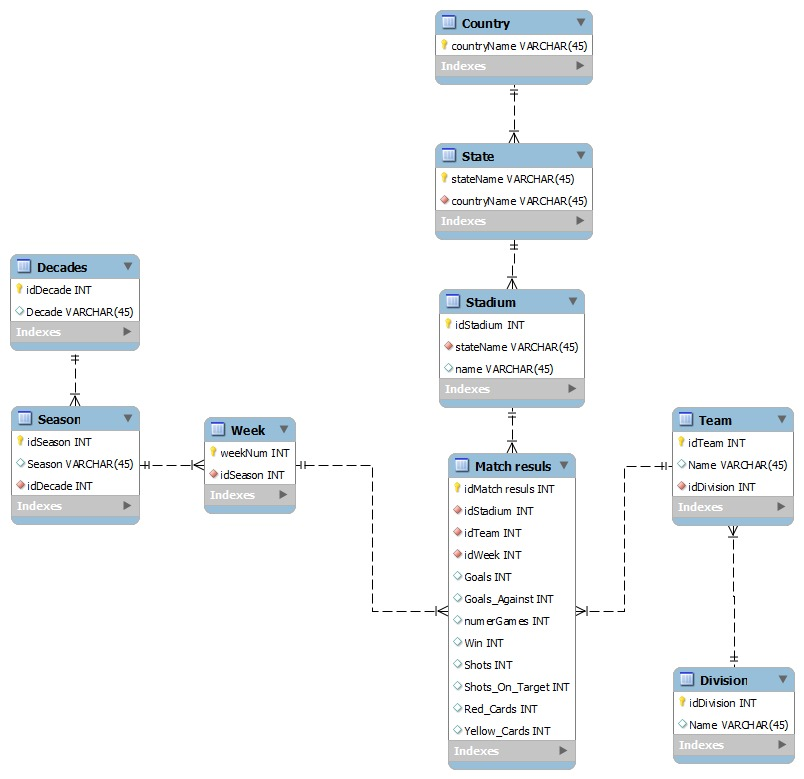
\includegraphics[width=1.0\columnwidth]{images/Snowflake}
	\caption{Snowflake Schema}
	\label{fig:probov}
\end{figure}
%

It’s follows a description of some columns:

\begin{itemize}
  \item countyName: Name of the country -> Germany
  \item stateName: Name of the state -> Baden-Württemberg, Rheinland-Pfalz
  \item idStadium: Stadium identification -> Allianz Arena
  \item idTeam: Unique team name -> FC Bayern Münich 
  \item idDivision: which division -> 1. Bundesliga
  \item weekNum: Play day in german is called week -> 2. Play day = 2. Week 
  \item idSeason: season 18/19 
\end{itemize}

But since the purpose of a Data Warehouse is also to make queries quicker and simpler, we extracted the data from the data warehouse into a data mart which looks like this:

\begin{figure}[htb]
	\centering
		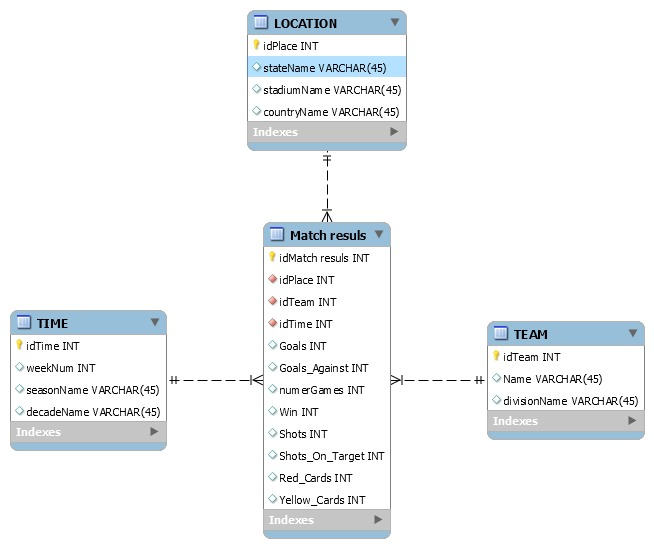
\includegraphics[width=1.0\columnwidth]{images/datamart}
	\caption{Data Mart}
	\label{fig:probov}
\end{figure}

%%%%%%%%%%%%%%%%%%%%%%%%%%%%%%%%%%%%%%%%%%%%%%%%%%%%%%%%%%%%%%%%%%%%%%%%%%%%%%%%%%%%%%%%%%%%%%%%%%%%%%%%%%%%%%%%%%%%%%%%%%%%%%%%
\section{Going from raw data to useful information} \label{sec:transf}
	
Once the raw data had been uploaded to a MySQL server and transformed in a staging database, the CDWH and DM had to be set up and their tables
properly structured, linked according to existing data contained in the staging area and knowledge on range of the data set. SQL scripts were 
created and executed to carry out this labour. 

On the data mart database, views were created to query for commonly interesting information, such as: How well does a team do depending on where
they play? Are they better when playing home or is it neglectable? How do teams perform per season?

The result of these queries were imported using Microsoft Excel to create pivot tables and generate charts to perform analytics.

\section{Result} \label{sec:further}
Here i will descripe our I

\begin{figure}[htb]
	\centering
		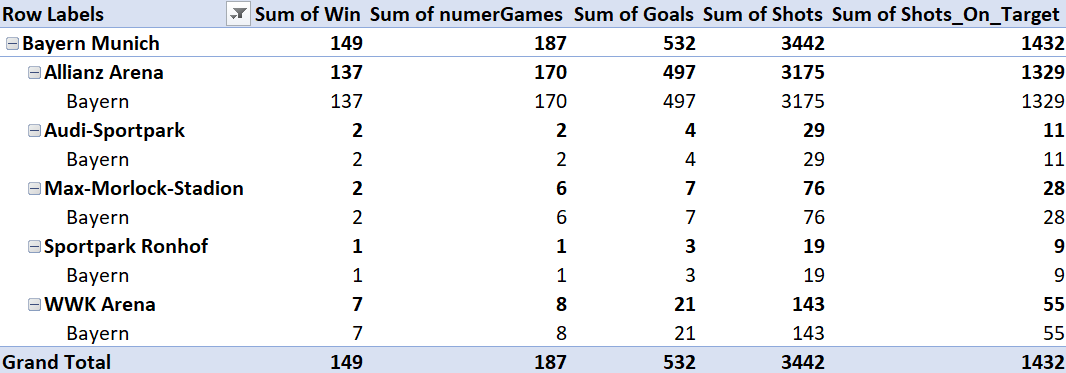
\includegraphics[width=1.0\columnwidth]{images/Pivot_Performance_Teams_Per_LocHomeAndAway_StateBayern}
	\caption{Performance of the Team Bayern Munich per Location }
	\label{fig:probov}
\end{figure}
\begin{figure}[htb]
	\centering
		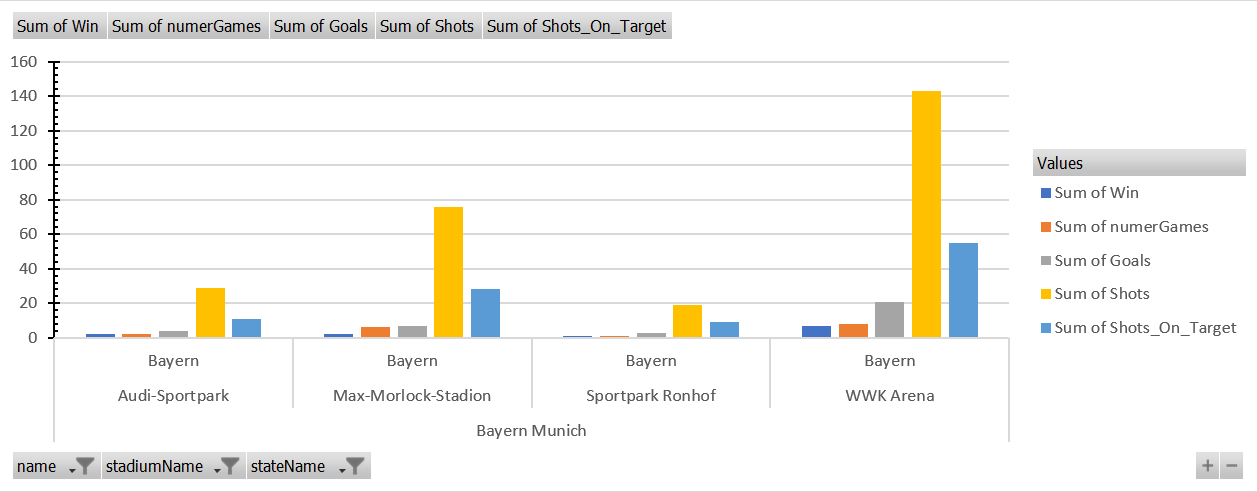
\includegraphics[width=1.0\columnwidth]{images/Chart_Performance_Teams_Per_LocAway_StateBayern}
	\caption{Performance of the Team Bayern Munich away from Home}
	\label{fig:probov}
\end{figure}
\begin{figure}[htb]
	\centering
		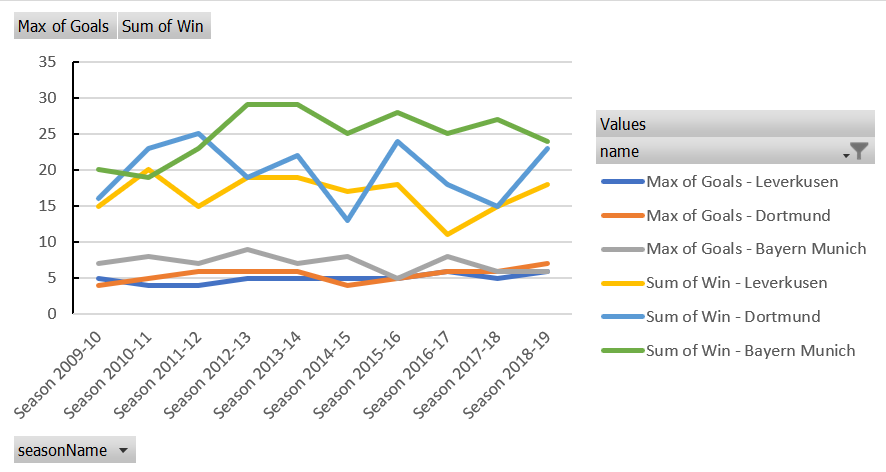
\includegraphics[width=1.0\columnwidth]{images/Chart_Performance_Teams_Per_Season}
	\caption{Performance of the Teams per Season}
	\label{fig:probov}
\end{figure} 
%%%%%%%%%%%%%%%%%%%%%%%%%%%%%%%%%%%%%%%%%%%%%%%%%%%%%%%%%%%%%%%%%%%%%%%%%%%%%%%%%%%%%%%%%%%%%%%%%%%%%%%%%%%%%%%%%%%%%%%%%%%%%%%%
\section{Conclusion} \label{sec:concl}
We have shown in this paper that the raw data is used to create a Data Warehouse, a data mart and also a detailed analysis with MySQL. We have check the data quality and have been reduced to the relevance of data needed for the Project. The data can be managed effectively and the analysis can be created. With our Data Warehouse it’s possible to create a forecast of a new game with information about the games from the last seasons. With this information we can get easily and compact understandable information about the matches, goals, red- and yellow cards and shots. Additionally, it’s necessary to say which team has a chance of winning a tournament or which team can win the game at home or away from home. The Project was for our team a new experience and the first insight in the development from a big dataset to make a data warehouse with the focus on the reduced data. This insight was for our team a good experience. 

%%%%%%%%%%%%%%%%%%%%%%%%%%%%%%%%%%%%%%%%%%%%%%%%%%%%%%%%%%%%%%%%%%%%%%%%%%%%%%%%%%%%%%%%%%%%%%%%%%%%%%%%%%%%%%%%%%%%%%%%%%%%%%%%
%%%%%%%%%%%%%%%%%%%%%%%%%%%%%%%%%%%%%%%%%%%%%%%%%%%%%%%%%%%%%%%%%%%%%%%%%%%%%%%%%%%%%%%%%%%%%%%%%%%%%%%%%%%%%%%%%%%%%%%%%%%%%%%%
% see file Literatur/bibliography!
\bibliographystyle{plaindin}
\bibliography{bibliography}

\end{document}
